%学会発表レジュメ ver. 1.0

\documentclass[uplatex,twocolumn]{jsarticle}
\usepackage[top=20mm,bottom=20mm,left=20mm,right=20mm]{geometry}
\usepackage[T1]{fontenc}
\usepackage{txfonts}
\usepackage{wrapfig}
\usepackage{multicol}
\usepackage[expert,deluxe]{otf}
\usepackage[dvipdfmx,hiresbb]{graphicx}
\usepackage{here}

\makeatletter

  \renewcommand{\section}{%
    \if@slide\clearpage\fi
    \@startsection{section}{1}{\z@}%
    {\Cvs \@plus.5\Cdp \@minus.2\Cdp}% 前アキ
    {.5\Cvs \@plus.3\Cdp}% 後アキ
    %{\normalfont\Large\headfont\raggedright}}
    {\normalfont\raggedright}}

  \renewcommand{\subsection}{\@startsection{subsection}{2}{\z@}%
    {\Cvs \@plus.5\Cdp \@minus.2\Cdp}% 前アキ
    {.5\Cvs \@plus.3\Cdp}% 後アキ
    %{\normalfont\large\headfont}}
    {\normalfont}}

  \renewcommand{\subsubsection}{\@startsection{subsubsection}{3}{\z@}%
    {\Cvs \@plus.5\Cdp \@minus.2\Cdp}%
    {\z@}%
    %{\normalfont\normalsize\headfont}}
    {\normalfont}} 
    
    
 \newenvironment{figurehere}
    {\def\@captype{figure}}
    {}    
    
\makeatother
%ここから上を編集する必要はない.(figure,を追加)


%footnotemarkで脚注の追加
\title{\vspace{-14mm}GitHub上のソフトウェア開発のためのフロー推薦手法 \footnotemark[0]}
\author{若月 純 \footnotemark[2] 矢吹 太朗 \\ 千葉工業大学 社会システム科学部 プロジェクトマネジメント学科\footnotemark[2]}
\date{}%日付を入れる必要はない.
\pagestyle{empty}
\begin{document}



\twocolumn[
	\maketitle
]
\begingroup
\def\thefootnote{\fnsymbol{footnote}}
\footnotetext[0]{Workflow recommendation method for software development on GitHub}
\footnotetext[2]{Jun WAKATSUKI・Department of Project Management, Social System Sciences, Chiba Institute of Tchnology}
\endgroup

\section{研究の背景}

ソフトウェア開発では,複数のメンバが同時に開発を行うため,ファイルの最新バージョンが分からなくなる,同一ファイルに対する変更が競合する等の問題が発生する.このような問題を解決するため,バージョン管理システムを用いる.バージョン管理システムとは,変更履歴を管理するシステムのことである\cite{ikeda2014}.

バージョン管理システムを提供するサービスに,GitHubがある.GitHubは,バージョン管理システムに加え,branch,Pull Requestといった開発を補助する機能を提供するサービスである.branchとは,履歴を分岐して記録していくためのものである.branchを用いることにより,同一リポジトリ内で,別々の作業を並行して行うことが出来るようになる.Pull Requestとは,自分のリポジトリから相手のリポジトリへ,変更を取り込んでもらうための要求を出す機能である.Pull Requestを用いることにより,変更が追加される前に確認することが出来る.

GitHubを使用する手順を開発フローと呼ぶ.現在わかっている開発フローの数は13個ある\cite{onodera2015}.開発フローの例を2つあげる.
GitHub Flowは,作業をするbranchを作成し,完成したら統合する.といった開発フローである.この開発フローはとてもシンプルなため,開発フローを実施するまでの学習コストは抑えられるが,開発規模が大きい場合,Pull Requestがたまりやすく,コードレビューに時間がかかってしまうことがある.
Git Flowは,develop branchから作業用branchを作成する.完成したらPull Requestを行い,作業用branchをdevelop branchに統合する.リリースができるレベルになったら,リリース用branchを作成し,作業をする.リリース作業が終了するとmasterブランチに統合され,バージョンタグを打ってリリースする.といった開発フローである.branch別にやることが決まっているため管理は容易であるが,branchが複数あるため,Pull Requestを異なったbranchに送ってしまう等の人的ミスが発生する場合がある\cite{ohtsuka2014}.

このように開発フローは,メリットとデメリットがある.しかし,選択する基準は定められていないため,状況にあった開発フローを選択するのは難しい。そのため、適切でない開発フローを選択し,開発に悪影響を与える危険がある.このような事態を防ぐため,適切な開発フローを選択できるようにするための指標が求められる.

本研究では、GitHub上の32件のプロジェクトを対象に、採用されている開発フローと、開発フローの採用に関わると思われる48の調査結果を解析した。
その結果、プロジェクトの性質に応じて,開発フローを推薦する手法を確立した。

\section{研究の目的}

GitHubを用いたソフトウェア開発プロジェクトの性質において,適切な開発フローを選択できるようにするための基準を提供する.

\section{プロジェクトマネジメントとの関連}

ソフトウェア開発プロジェクトにおいて,プロジェクトマネージャーは,QCDを達成させるためにスケジュール,コスト,品質コントロールを行う.これらのコントロールを,GitHubを用いた開発フローを導入し,テストを自動化したり,誤操作を防いだりすることで補助することが出来る.

\section{研究の方法}


本研究は3段階に分かれる.
\begin{enumerate}
\item GitHub上のプロジェクトから,採用されている開発フローと、開発フローの採用に関わると思われる項目を調査する.
\item 調査結果を解析する.
\item 解析結果の精度と再現率を求める. 
\end{enumerate}

初めに,GitHub 上のプロジェクトから,開発フローと開発フローの採用に関わると思われる項目を調査する.
開発フローは,GitHub上のbranch,Pull Requestの特性から求められる.branchにstableが用いられている場合は,Stable Flowである.master branchから記述的な名前のbranchがある場合は,GitHub Flowである.develop branchとrelease branchがある場合は,Git Flowである.バージョンごとにbranchが作られている場合は,LINE Flowである. Pull Request にWIPがある場合は,WIP Flowである.
開発フローの採用に関わると思われる項目は、GitHub上のデータを用いる。GitHub上のデータは,GitHubブラウザに載っているデータと載っていないデータがある.載っていないデータは,リポジトリをクローンして調査する.

次に,調査したデータを分析する.
調査したデータの分析は,決定木分析を行う.決定木分析により,プロジェクトがどのような性質を持つときに,どの開発フローが使われているかを明らかにする.

最後に,解析結果の精度と再現率を求める。
調査したデータをランダムに22件と10件の2種類に分ける。
22件のデータで決定木分析を行う.决定木分析結果と10件のデータを照らし合わせて、決定木の精度と再現率を調べる。
これを10回行い,信頼度95\%区間の精度と再現率を用いる.


\section{成果物のイメージ}

調査データを用いて决定木分析を行い,開発フローを選択する基準を求める.
選択する基準は,次に書く例のように定量的になっている.
人数が5人以上の時かつ,使われている言語がRubyの時は,GitHub Flowを選択する.

また,選択する基準の精度と再現率を求める.
精度と再現率は50\%以上になることを目指す.


\section{現在の進捗状況}

% 大文字のHを使用することで好きな位置に図を配置
\begin{figure}[H]
%\includegraphics[width=図の幅,clip]{ファイル名}\label{参照用ラベル}
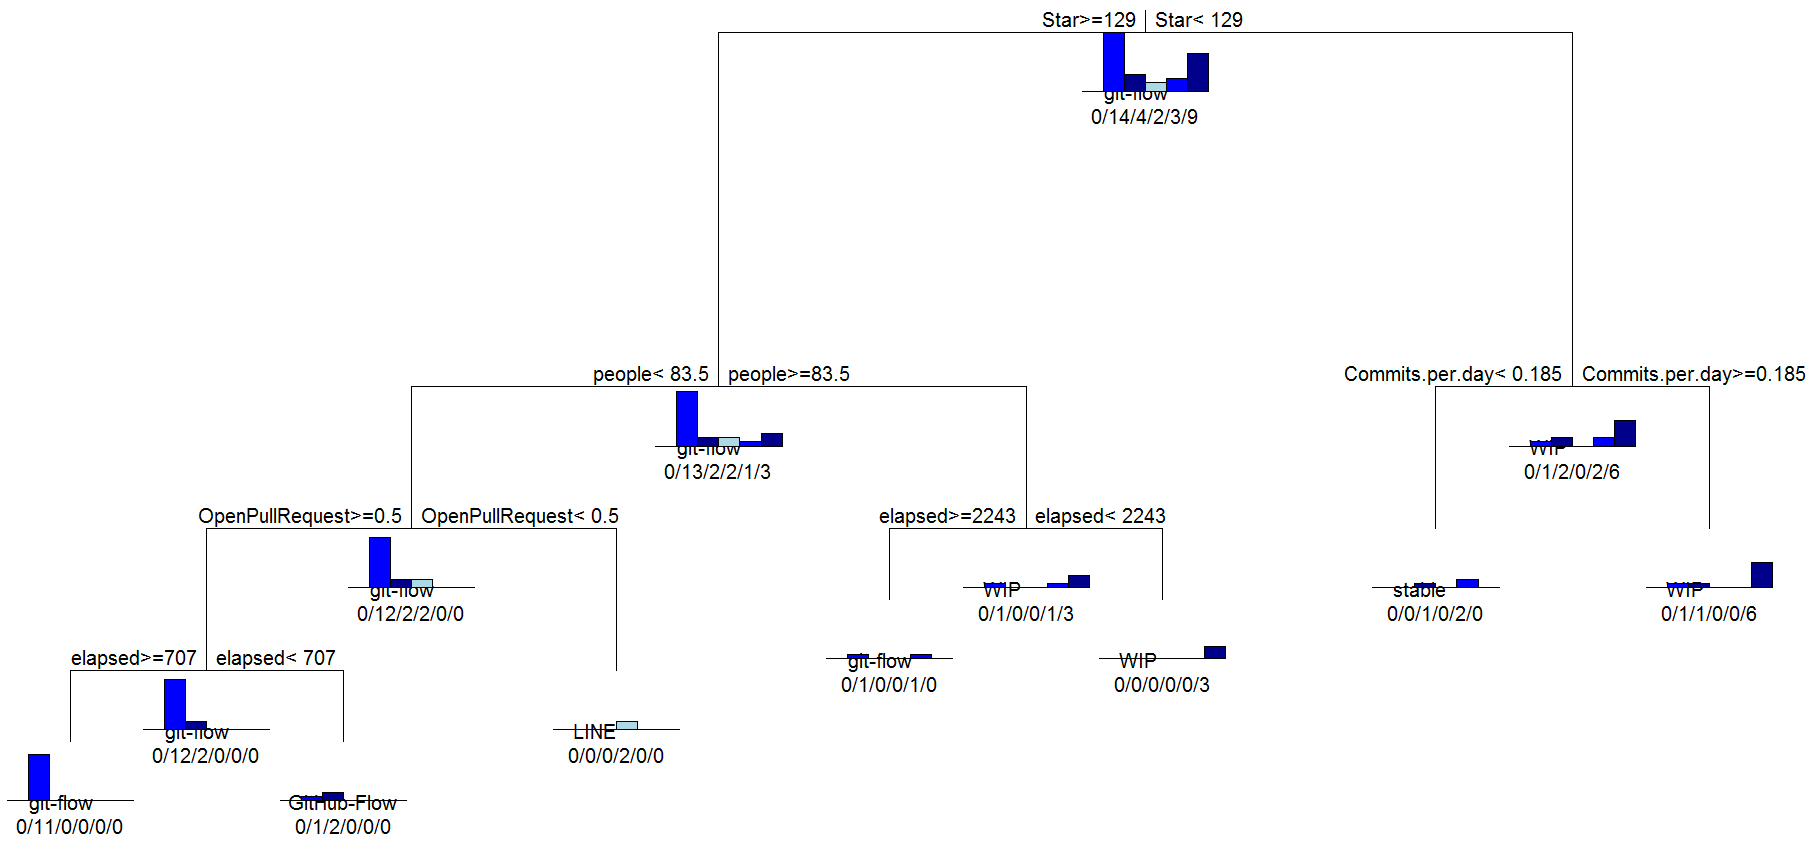
\includegraphics[width=8.5cm,clip]{images.png}
\caption{プロジェクトの性質により選択される開発フローの違い}\label{決定木}
\end{figure}


GitHub上の32個のプロジェクトから,プロジェクトの性質と開発フローを調査し,決定木分析を行った.また,決定木分析結果の精度と再現率を求めた。


プロジェクトの性質は,プロジェクト経過日数,行数,ファイル数,バイト数,Watch 数,Star 数,Fork 数,Commit数,branch 数,Release 数,人数,Open Issues 数,Closed Issues 数,Issues 数,Open PullRequest数,Closed PullRequest数,PullRequest数,Label 数,Open Milestone 数,Closed Milestone 数,Milestone 数,Wiki 数.開発人数,言語,一日あたりの行数とCommit数,1人日あたりの行数とCommits数を調査した.
言語は26種類の項目を作成し、プロジェクトで使用している場合1,使用していない場合0で判別した。


開発フローは,Git Flow,GitHub Flow,LINE Flow,Stable Flow,WIP Flowの5種類だった.

決定木分析結果は,図1である.分析結果から,プロジェクトの性質により選択される開発フローが明らかにされた.
この決定木は,全データをまずStar数で分類している.Star数とは,注目度を表す指標である.
star数が多い場合git flow,star数が少ない場合、wip flowが多く選択されている。
ここから、常にチェックしているユーザが多いプロジェクトの場合,主にbranchで管理し,
常にチェックしているユーザが少ないプロジェクトの場合,主にPull Requestで管理していることが言える.


决定木の精度と再現率について記述する.
精度の平均は41\%,95\%信頼区間は26\~56\%だった.
再現率の平均は51\%,95\%信頼区間は29\~73\%だった.


\section{今後の課題}
この分析で,一日あたりの行数とCommit数,1人日あたりの行数とCommits数は,平均を用いている.
プロジェクトの傾向を考慮していないため,特定の曜日にCommitが増える場合や,Pull Requestを確認する日等がある場合でも同様のフローになってしまう.
そのため,より詳細なプロジェクトの傾向を調査し,分析を行えば,决定木の精度と再現率をあげられると考える.



\bibliographystyle{junsrt}
\bibliography{biblio}%「biblio.bib」というファイルが必要.


\end{document}